%%%%%%%%%%%%%%%%%%%%%%%%%%%%%%%%%%%%%%%%%%%%%%%%%%%%%%%%%%%%%%%%%%%%%%%%%%%%%%%%
%2345678901234567890123456789012345678901234567890123456789012345678901234567890
%        1         2         3         4         5         6         7         8

% \documentclass[a4paper, 10pt, conference]{ieeeconf}      % Use this line for a4 paper
\documentclass[journal,twoside,web]{ieeecolor}
\usepackage{orcidlink}
\usepackage{lcsys}
\usepackage{amsmath,amssymb,amsfonts} % assumes amsmath package installed
\usepackage{bm}

\newtheorem{assumption}{Assumption}
\newtheorem{theorem}{Theorem}
\newtheorem{corollary}{Corollary}[theorem]
\newtheorem{remark}{Remark}
\newtheorem{lemma}{Lemma}
\newtheorem{proposition}{Proposition}
\newtheorem{definition}{Definition}
\newtheorem{problem}{Problem}

%%%%%%%%%%%%%%%%%%%%%%%%%%%%%%%%%%%%%%%%%%%%%%%%%%%%%%%%%%%%%%%%%%%%%%%%%%%%%%%%
\usepackage{mathtools}
%%%%%%%%%%%%%%%%%%%%%%%%%%%%%%%%%%%%%%%%%%%%%%%%%%%%%%%%%%%%%%%%%%%%%%%%%%%%%%%%
%%%%% For the references above equality and others relationships in equations
%%%%%%%%%%%%%%%%%%%%%%%%%%%%%%%%%%%%%%%%%%%%%%%%%%%%%%%%%%%%%%%%%%%%%%%%%%%%%%%%
\newcounter{relctr} %% <- counter for relations
\everydisplay\expandafter{\the\everydisplay\setcounter{relctr}{0}} %% <- reset every eq
\renewcommand*\therelctr{\alph{relctr}} %% <- label format
%%%%%%%%%%%%%%%%%%%%%%%%%%%%%%%%%%%%%%%%%%%%%%%%%%%%%%%%%%%%%%%%%%%%%%%%%%%%%%%%
\newcommand\labelrel[2]{%
  \begingroup
    \refstepcounter{relctr}%
    \stackrel{\textnormal{(\alph{relctr})}}{\mathstrut{#1}}%
    \originallabel{#2}%
  \endgroup
}
\AtBeginDocument{\let\originallabel\label} %% <- store original definition
%%%%%%%%%%%%%%%%%%%%%%%%%%%%%%%%%%%%%%%%%%%%%%%%%%%%%%%%%%%%%%%%%%%%%%%%%%%%%%%%

\title{Wireless Control With Channel State Detection And Message Dropout Compensation}

\author{Yuriy \textbf{Zacchia Lun}\,\textsuperscript{\orcidlink{0000-0002-9408-8773}},\,\IEEEmembership{Member, IEEE}, Fortunato \textbf{Santucci}\,\textsuperscript{\orcidlink{0000-0002-0229-6277}},\,\IEEEmembership{Senior Member, IEEE},\\ and Alessandro \textbf{D'Innocenzo}\,\textsuperscript{\orcidlink{0000-0002-5239-0894}},\,\IEEEmembership{Member, IEEE}
\thanks{The authors are with the 
Department of Information Engineering, Computer Science and Mathematics (DISIM), University of L'Aquila, L'Aquila 67100, Italy. (e-mail addresses:
        {yuriy.zacchialun@univaq.it},\\ {fortunato.santucci@univaq.it}, and {alessandro.dinnocenzo@univaq.it})}%
}

\def\BibTeX{{\rm B\kern-.05em{\sc i\kern-.025em b}\kern-.08em
    T\kern-.1667em\lower.7ex\hbox{E}\kern-.125emX}}
\markboth{\journalname, VOL. XX, NO. XX, XXXX}
{Zacchia Lun \MakeLowercase{\textit{et al.}}: Wireless Control With Channel State Detection And Message Dropout Compensation}

\begin{document}

\maketitle
\thispagestyle{empty}
\pagestyle{empty}

%%%%%%%%%%%%%%%%%%%%%%%%%%%%%%%%%%%%%%%%%%%%%%%%%%%%%%%%%%%%%%%%%%%%%%%%%%%%%%%%
\begin{abstract}
This letter presents a framework for designing optimal state-feedback control that uses a wireless actuation link with imperfect channel state information to transfer the current and future control inputs that actuators can apply if future control messages are lost. The dropout compensation strategy supports scaling inputs to actuators when necessary. We analytically solve finite- and infinite-horizon control problems and present a necessary and sufficient stability condition for any given infinite-horizon state-feedback control law. We validate the results using an illustrative example.
\end{abstract}
\begin{keywords}
Control over communications, Markov processes.
\end{keywords}
%%%%%%%%%%%%%%%%%%%%%%%%%%%%%%%%%%%%%%%%%%%%%%%%%%%%%%%%%%%%%%%%%%%%%%%%%%%%%%%%
\section{Introduction}\label{sec:intro}
\IEEEPARstart{W}{ireless} networked control systems (WNCSs), with their mission-critical applications in intelligent transportation, industrial automation, smart grids, and telesurgery, are a significant area of interest for both industry and academia, as highlighted in \cite{park2018comm,liu2021iot}, and \cite{pezzutto2024arc}. Estimation and control over unreliable links are key topics of WNCS research, as discussed in \cite{park2018comm,pezzutto2024arc,yZL-2025-automatica}, and references therein. 

An essential research outcome of \cite{yZL-2025-automatica} and \cite{impicciatore2024tac} is that accurate and timely knowledge of the communication link conditions can substantially improve closed-loop performance. However, perfect wireless channel state information (CSI) may be difficult to achieve in realistic communication scenarios, so only imperfect or statistical CSI may be available in practice, see \cite{zheng2022survey}, \cite{pourkabirian2021robust}, and \cite{akgun2024interference}. Another potential limitation of the results in \cite{yZL-2025-automatica} and \cite{impicciatore2024tac} is computing and transmitting only the current control input. The model predictive control (MPC)-based algorithms outlined in \cite{pezzutto2024arc} instead rely on transferring a sequence of future control inputs that actuators can use if future control messages are lost. This approach increases processing and transmission delays, message loss probabilities, and network traffic due to message size growth. The number of future control inputs to transfer becomes a significant design parameter, balancing the adverse effects of increased message size and the benefits of improved control inputs. This letter presents a framework for studying this trade-off under imperfect CSI and a hybrid message dropout compensation (MDC) scheme that combines transmitting multiple control inputs and scaling inputs to actuators when necessary.
We incorporate CSI uncertainties using the detector-based approach of \cite{costa2015detector} and \cite{deoliveira2018mixed}, which we extend to the one-time-step delayed channel state observation setting of \cite{yZL-2025-automatica} and \cite{impicciatore2024tac}, where finite-state Markov channels (FSMCs, see \cite{sadeghi2008finite}) model the dynamics of wireless links. Thus, we substantially extend the results of \cite{yZL-2025-automatica} to a highly general unconstrained setting.

The \textit{contribution} of this letter is threefold.
\begin{enumerate}
    \item We present a practical hidden Markov jump linear system (HMJLS) model of discrete-time linear stochastic systems with hybrid MDC and imperfect CSI.
    \item We derive finite- and infinite-horizon linear–quadratic regulators %\textcolor{blue}{(LQRs)} 
    and introduce a necessary and sufficient stability condition for any given infinite-horizon state-feedback (SF) control law that requires computing the spectral radius of a stability verification matrix.
    \item We validate the theoretical results on numerical examples showcasing the impact of the number of transmitted anticipative control inputs and CSI uncertainties.
\end{enumerate}

\textit{Notation:} $\mathbb{R}$, $\mathbb{Z}^{+}$, and $\mathbb{Z}^{0+}$ indicate the sets of reals and positive and nonnegative integers. $\mathbb{R}^{n}$ indicates the $n$-dimensional Euclidean space. The symmetric positive definite and positive semidefinite matrices $Z$ are denoted by $Z\succ 0$ and $Z\succeq 0$. $Z^{\top}$ indicates the transpose of a matrix $Z$. $\rho(Z)$ is the spectral radius of a square matrix $Z$. 
$\mathbb{P}$ represents the probability of an event, and $\mathbb{E}$ denotes the expected value of a random variable. $I_N$ indicates the identity matrix of size $N$. 

Throughout this letter, $N$ indicates the number of FSMC states, and $M$ is the number of detector outputs, with $M\leq N$.
Furthermore, $e_i$ denotes the column vector of the standard basis of $\mathbb{R}^{N}$: all its components are zero except the $i$th, which equals one. The column vectors of the standard basis of $\mathbb{R}^{M}$ are denoted by $\hat{e}_{\mu}$, with $\mu\in\mathbb{Z}^{+}$, $\mu\leq M$. In addition, $\oplus$ indicates the direct sum that produces a diagonal matrix with the addends becoming elements on the main diagonal. $\otimes$ is the Kronecker product. Finally, $\mathbf{0}$ and $\mathbf{1}$ are vectors of appropriate size with all elements equal to zero and one, respectively.

This letter is \emph{organized} as follows. 
Section \ref{sec:prelim} presents the preliminaries and motivation examples for the practical use of the detector-based approach.
Section \ref{sec:model} formalizes the system model and defines the control problem.
Section \ref{sec:hmjls} introduces an equivalent model of the closed-loop system.
Sections \ref{sec:lqr-fh}, \ref{sec:stability}, and \ref{sec:lqr-ih} address the finite-horizon optimal SF control, closed-loop system stability, and infinite-horizon optimal SF control, respectively.
Section \ref{sec:example} validates the results in a numerical example, and 
Section \ref{sec:conclusions} concludes the letter.

\section{Preliminaries and Motivation Example}\label{sec:prelim}
In a WNCS setting, controllers use wireless links to transmit control messages to actuators. 
Similarly, sensors transmit their measurements to controllers wirelessly. Wireless links exhibit a time-varying behavior captured well by FSMC models. 

Any FSMC has a finite set of states $\mathcal{S}\triangleq\{s_i\}_{i=1}^{N}$. Each state can be characterized by predefined signal-to-interference-plus-noise ratio (SINR) thresholds and a corresponding packet dropout probability \cite{zacchialun2024access}. A discrete-time Markov chain $\{\theta_k\}$ dictates the active channel state, whose packet dropout probability and transition probabilities (TPs) depend on the SINR dynamics. We formally define an FSMC as follows: $\forall k\in \mathbb{Z}^{0+}$,
\begin{equation}\label{eq:p-ij}
    \mathbb{P}(\theta_{k} = s_j \mid \theta_{k-1} = s_i) = p_{ij} \geq 0,~ \sum_{j=1}^N p_{ij} = 1,
\end{equation}
\begin{equation}\label{eq:p-delta}
    \mathbb{P}(\delta_k = 1 \mid \theta_{k} = s_j) = \hat{\delta}_{j},~
    \mathbb{P}(\delta_k = 0 \mid \theta_{k} = s_j) = 1 - \hat{\delta}_{j},
\end{equation}
where $\{\delta_k\}$ is a binary stochastic process that models the packet loss between transmitter and receiver.

For notational convenience, we group
channel state TPs in the transition probability matrix (TPM) $P_{c}^{} \triangleq [p_{ij}]_{i,j=1}^{N}$
and the  success (or, conversely, failure) probabilities of delivering a packet at time $k$ in the following matrices:
\begin{equation}\label{eq:Ps}
    P_{s}^{} \triangleq [p_{ij}\hat{\delta}_{j}]_{i,j=1}^{N},~P_{f} = P_{c} - P_{s}.
\end{equation}
We also indicate the channel state probability at time $k$ as
\begin{equation}\label{eq:pik}
     \mathbb{P}(\theta_{k} = s_i) = \pi_{i}(k).
\end{equation}

Wireless receivers perform CSI measurements that may be fed back to the transmitters. In the sensing links, the controller is the receiver with direct access to the measured CSI. In the actuation links, the controller is the transmitter. It can typically access the measured CSI using a reporting mechanism similar to acknowledgment (ACK) of transmission outcomes, which introduces a delay. This delay makes the optimal SF control problem the main challenge in the unconstrained output feedback control over FSMC links \cite{impicciatore2024tac}. Consequently, this letter focuses on the unconstrained SF control problem that explores the impact of the actuation link's CSI measurement noise, including particular cases of partial or no observation of FSMC states. We adopt the detector-based approach as follows.

Let $\hat{\theta}_k \in \{\hat{s}_{\mu}\}_{\mu=1}^{M}$ denote the measured CSI, which is the output of a detector with an emission probability matrix (EPM)
\begin{subequations}\label{eq:epm-alpha}
\begin{equation}\label{eq:epm}
    P_{e}^{} \triangleq \left[\alpha_{i\mu}\right]_{i,\mu=1}^{N,M},
\end{equation}
\begin{equation}\label{eq:alpha}
   \mathbb{P}(\hat{\theta}_{k} = \hat{s}_{\mu} \mid \theta_{k} = s_i) = \alpha_{i\mu} \geq 0,~ \sum_{i=1}^N \alpha_{i\mu}= 1.
\end{equation}
\end{subequations}

$M\leq N$ encompasses the following particular cases:
\begin{itemize}
    \item \emph{Perfect CSI}: $M=N$ and $P_e = I_N$ so that %$\hat{\theta}_k = \theta_k ~\forall k$, i.e., 
    $\theta_k$ is known.
    \item \emph{No CSI}: $M=1$ and $P_e = \mathbf{1}$ so that $\theta_k$ is unknown.
\end{itemize}
Furthermore, the case of partial observation with clusters is also well represented by a detector with $M<N$, see \cite{costa2015detector}.

In the WNCS setting, we can rely on CSI based on SINR measurements $\hat{\gamma}_k$, where $\hat{\theta}_k = \hat{s}_{\mu} \Leftrightarrow\hat{\gamma}_k\in [\hat{\beta}_{\mu-1},\hat{\beta}_{\mu})$, with $\hat{\beta}_{\mu-1}$ and $\hat{\beta}_{\mu}$ indicating the detector's SINR thresholds. Since $\hat{\gamma}_k \in [0,+\infty)$, $\hat{\beta}_0 = 0$, and $\hat{\beta}_{M}=+\infty$. CSI measurements may be affected by measurement noise $\omega_k$, i.e., 
\begin{equation}\label{eq:gamma-hat}
    \hat{\gamma}_k = \gamma_k + \omega_k,
\end{equation}
where $\gamma_k$ denotes the nominal SINR that drives the FSMC: 
$\theta_k = s_{i} \Leftrightarrow\gamma_k\in [\beta_{i-1},\beta_{i})$, where $\beta_{i-1}$ and $\beta_{i}$ are the SINR thresholds of a FSMC. $\gamma_k \in [0,+\infty)$, $\beta_0 = 0$, and $\beta_{N}=+\infty$.

As a \emph{motivation example} with significant practical relevance, we consider $\omega_k \sim \mathcal{N}(0,\sigma_{\omega}^2)$ and $M\leq N$. 
Depending on the characteristics of the wireless propagation environment, $\gamma_k$ can have lognormal, Rayleigh, Rice, or Nakagami distributions \cite{stuber2017principles}. 
Let $f_{\gamma}(z)$ be the probability density function of $\gamma_k$.
\begin{equation}\label{eq:alpha-normal}
    \alpha_{i\mu} = \frac{
    \int_{\beta_{i-1}}^{\beta_{i}}\left(
    \mathcal{Q}\left(\frac{\hat{\beta}_{\mu-1}-z}{\sigma_{\omega}}\right) - 
    \mathcal{Q}\left(\frac{\hat{\beta}_{\mu}-z}{\sigma_{\omega}}\right) 
    \right) f_{\gamma}(z)dz}{
    \int_{\beta_{i-1}}^{\beta_{i}} f_{\gamma}(z)dz},
\end{equation}
where $\mathcal{Q}(\cdot)$ indicates the Q-function. For any given $\sigma_{\omega}$, $f_{\gamma}(z)$, and % sets of \textcolor{magenta}{inner} 
thresholds $\{\hat{\beta}_{\mu}\}_{\mu=1}^{M-1}$ and $\{\beta_{i}\}_{i+1}^{N-1}$, the values of $\alpha_{i\mu}$ can be found numerically using \eqref{eq:alpha-normal}.

For notational convenience, we define the diagonal matrices
\begin{equation}\label{eq:diag-prob}
     P_{\pi}^{}(k) = \bigoplus_{i=1}^{N} \pi_{i}(k),~P_{\alpha}^{}(\mu) = \bigoplus_{i=1}^{N} \alpha_{i\mu}.
\end{equation}

\section{System Model and Problem Definition}\label{sec:model}
In this letter, we consider a discrete-time linear system % in the standard state-space form
\begin{equation}\label{eq:state}
        x_{k+1} = A x_{k} + B u_{k}^{} + w_{k},
\end{equation}
where $\forall k \!\in\! \mathbb{Z}^{0+}$, $x_k\!\in\!\mathbb{R}^{n_x}$ and $u_k^{}\!\in\!\mathbb{R}^{n_u}$ are the system state and control input to actuators, $A$ and $B$ are state and input matrices of appropriate size, and $w_k\!\in\!\mathbb{R}^{n_x}$ is a white Gaussian process noise having zero mean and covariance matrix $\Sigma_w$.

The controller sends a control message $\hat{u}_k$ comprising the current input and $n_{f}\in\mathbb{Z}^{0+}$ future inputs, to account for possible control message dropouts after the current transmission: 
\begin{equation}\label{eq:control-message}
    \hat{u}_k =
    \big([\bar{u}_{(k+f\mid k)}^{\top}]_{f=0}^{n_f}\big)^{\!\top} = 
    [\bar{u}_{(k\mid k)}^{\top},\dots,\bar{u}_{(k+n_f\mid k)}^{\top}]^{\top}.
\end{equation}

If the control message dropout interval is longer than the number of anticipated control inputs $n_f$, the actuators apply the generalized control MDC at the last available control input.  Specifically, this input is multiplied by a matrix $\mathit{\Phi}=\bigoplus_{i=1}^{n_u} \phi_i$, with $0 \leq \phi_i \leq 1$. 
The actuator inputs are obtained as follows.
\begin{equation}\label{eq:uk}
    u_k = F \tilde{u}_k,~F \triangleq \tilde{e}_{1}^{\top} \otimes I_{n_u},
\end{equation}
\begin{equation}\label{eq:uk-tilde}
    \tilde{u}_k = \delta_k \hat{u}_k + \left(1-\delta_k\right) H \tilde{u}_{k-1},~\tilde{u}_{-1} = \mathbf{0},
\end{equation}
\begin{equation}\label{eq:H}
    H \triangleq \sum_{i=1}^{n_f} \tilde{e}_{i} \otimes \tilde{e}_{i+1}^{\top} \otimes I_{n_u} + 
    \tilde{e}_{n_f+1} \otimes \tilde{e}_{n_f+1}^{\top} \otimes \mathit{\Phi}.
\end{equation}
$\tilde{e}_{i}$ indicates the column vector of the standard basis of $\mathbb{R}^{n_f+1}$.
$u_k$ in \eqref{eq:uk} extracts the first $n_u$ elements from the buffer $\tilde{u}_k$ described by \eqref{eq:uk-tilde}.
If a control message is received successfully, $\delta_k = 1$, and the buffer stores the message. Otherwise, the buffer performs a linear transformation of its content through the matrix $H$. This transformation deletes the first $n_u$ elements,  moves all the remaining elements by $n_u$ positions upwards, multiplies the last $n_u$ elements by $\mathit{\Phi}$, and stores the result at the bottom of the buffer. 

\textcolor{blue}{Fig.~\ref{fig:architecture} summarizes this closed-loop system architecture.}
\begin{figure}
\begin{center}
\vspace{5pt}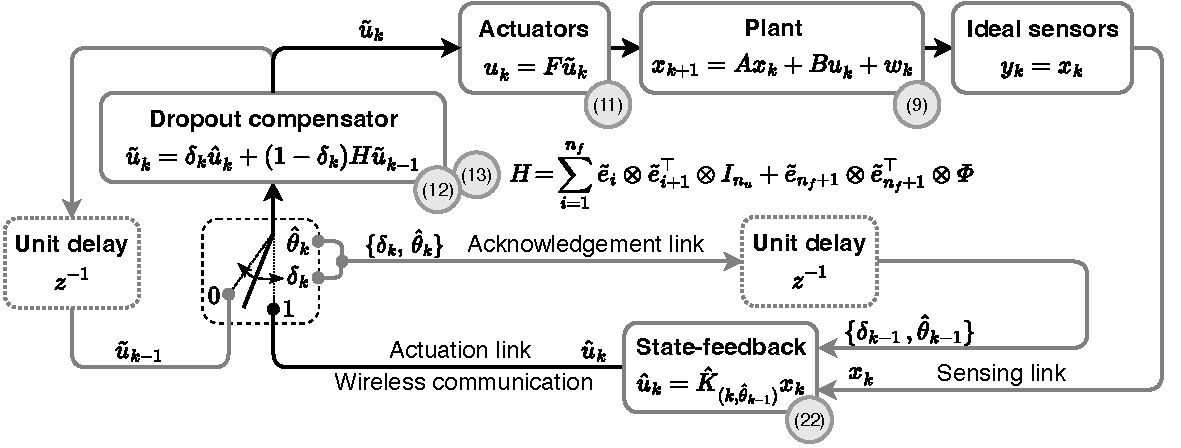
\includegraphics[width=\columnwidth]{./wncs-lcss-cdc-25-architecture.pdf}\vspace{-4pt}
\caption{\textcolor{blue}{The closed-loop system architecture. The square blocks indicate the main components, and the shaded circles reference the related equations. A wireless link delivers SF control inputs to the actuators. The receiver measures the link state $\theta_k$ and communicates the measurement $\hat{\theta}_k$ with the transmission outcome $\delta_k$ to the controller. }}\label{fig:architecture}
\end{center}
\end{figure}

\textcolor{blue}{Similar to} \cite{yZL-2025-automatica}, \cite{impicciatore2024tac}, and references therein, we make the following \emph{technical assumptions}:
\begin{enumerate}
	\item[A.1)] The initial conditions $x_0$ and $\theta_0$ are independent. % random variables.
	\item[A.2)] The process noise $\{w_k\}$ is independent of the initial state $x_0$ and the binary stochastic process $\{\delta_k\}$.
	\item[A.3)] The process noise $\{w_k\}$ and the discrete-time Markov chain $\{\theta_k\}$ are independent.
	\item[A.4)] %The Markov chain 
    $\{\theta_k\}$ is ergodic. Its steady-state probability distribution is $\bm{\pi}(\infty) = [\pi_{i}(\infty)]_{i=1}^{N}$, where $\pi_{i}(\infty) = \lim_{k\to\infty} \pi_{i}(k)$.
\end{enumerate}

The controller information set for the computation of the current and future control inputs in \eqref{eq:control-message} is the following.
	\begin{equation}\label{eq:info-set}
\mathcal{I}_{k} = \big\{
	\left(x_{t}\right)_{t=0}^{k}, 
	\left(\delta_{t-1}\right)_{t=1}^{k}, 
	(\hat{\theta}_{t-1})_{t=1}^{k} \big\}.
\end{equation}
In particular, the controller can obtain the CSI detected by the actuator's receiver, not the actual state of the FSMC. Moreover, as a transmitter, the controller does not measure CSI and cannot know the outcome of a control message transmission before sending it. This information comes from the actuator's receiver with a time-step delay.

Let $T\in\mathbb{Z}^{+} \cup \{\infty\}$ denote a control time horizon. $\bm{u}_{T}^{n_f}$ is a sequence of length $T$ of control messages as in \eqref{eq:control-message} such that
\begin{equation}\label{eq:control-element}
    \bar{u}_{(k+f\mid k)} = K_{(k+f,\hat{\theta}_{k-1})}x_k.
\end{equation}
$\mathcal{U}_{T}^{n_f}$ denotes the set of all possible sequences defined by $\bm{u}_{T}^{n_f}$.
The following optimization problem defines
the LQR (linear–quadratic regulation) paradigm:
\begin{equation}\label{eq:control-fin}
    \hat{\bm{u}}_{T}^{n_f} = \mathop{\mathrm{arg\,min}}_{\bm{u}_{T}^{n_f} \in \mathcal{U}_{T}^{n_f}} J_{T}^{}(x_0,\mathcal{U}_{T}^{n_f}),
\end{equation}
where $J_{T}^{}(\cdot)$ is a cost function defined as follows for any given pair of state-weighting and input-weighting matrices $Q\succeq 0$ and $R \succ 0$ of appropriate size.
For $T<\infty$,
\begin{equation}\label{eq:cost-def-fin}
    J_{T}^{}(x_0,\mathcal{U}_{T}^{n_f}) \!\triangleq \mathbb{E}(x_T^{\top} Q x_T +\! \sum_{k=0}^{T-1} x_k^{\top} Q x_k + u_k^{\top}Ru_k \mid \mathcal{I}_0).
\end{equation}
$J_{T}^{}(\cdot)$ weights the inputs to the actuators, which depend via \eqref{eq:uk}–\eqref{eq:H} on $\bm{u}_{T}^{n_f}$, $\{\delta_k\}$, and $\mathit{\Phi}$. For $T=\infty$, 
\begin{equation}\label{eq:cost-def-inf}
    J_{\infty}^{}(x_0,\mathcal{U}_{\infty}^{n_f}) = \limsup_{T\to\infty} \frac{1}{T} J_{T}^{}(x_0,\mathcal{U}_{T}^{n_f}).
\end{equation}

This letter solves the following design problem.

\begin{problem}\label{problem:lqr}
   Given a system \eqref{eq:state}–\eqref{eq:H}, design a controller that minimizes the cost \eqref{eq:cost-def-fin} or \eqref{eq:cost-def-inf} under assumptions A.1)–A.4) and the information set \eqref{eq:info-set}.
\end{problem}

To analytically solve the problem \eqref{eq:control-fin} in the FSMC setting with the measured CSI, we first derive an equivalent HMJLS representation of \eqref{eq:state}–\eqref{eq:H}, as detailed below. 

\section{Hidden Markov Jump Linear System Model}\label{sec:hmjls}
The system \eqref{eq:state}–\eqref{eq:H} trajectories depend on realizations of the stochastic process $\{\delta_k\}$. At time $k$, the controller sees the realizations of $\{\delta_k\}$ through ACK messages from actuators, which arrive with a delay of one step, as formalized by \eqref{eq:info-set}. 
We count the number of consecutive negative ACK messages in a stochastic variable $\mathit{\Delta}_{k}$:
\begin{equation}\label{eq:z-k}
    \mathit{\Delta}_{k}=(1-\delta_{k-1})(\mathit{\Delta}_{k-1}+1).
\end{equation}
\begin{equation}\label{eq:zl}
    \mathit{\Delta}_{k}=\ell\Leftrightarrow \delta_{k-1-\ell}=1 \land 
	\delta_{k-t}=0 ~ \forall t\in\mathbb{Z}^{+} : t\leq \ell.
\end{equation}
If $\ell\!=\!0$, then $\left\{t\right\}_{t=1}^{0} \!=\! \emptyset$, that is, $\mathit{\Delta}_{k}\!=\!0\Leftrightarrow \delta_{k-1}\!=\!1$.
Let $\mathcal{T}$ denote the set of time instances in which actuators successfully receive control messages: %. Formally, 
\begin{subequations}\label{eq:tau} 
\begin{equation}\label{eq:calT}  
    \mathcal{T} \triangleq \left\{ k : \delta_k = 1 \right\}_{k\in\mathbb{Z}^{0+}} = \{ \tau_{(m)}\}_{m\in\mathbb{Z}^{0+}}.
\end{equation}
From \eqref{eq:z-k}, \eqref{eq:zl}, and \eqref{eq:calT}, for all $m\in\mathbb{Z}^{0+}$,
\begin{equation}\label{eq:deltatau}
    \tau_{(m)} \in \mathcal{T}  \Rightarrow \delta_{\tau_{(m)}} = 1 \Rightarrow \mathit{\Delta}_{\tau_{(m)}+1} = 0,
\end{equation}
\begin{equation}\label{eq:tau+}
    \tau_{(m+1)} = \tau_{(m)} + 1 + \mathit{\Delta}_{\tau_{(m+1)}}.
\end{equation}
\end{subequations}
From \eqref{eq:control-message} and \eqref{eq:control-element}, 
\begin{equation}\label{eq:control-gains-matrix}
    \hat{u}_{k} = \hat{K}_{(k,\hat{\theta}_{k-1})} x_k,~~
    \hat{K}_{(k,\hat{\theta}_{k-1})}^{\top} = \left[K_{(k+f,\hat{\theta}_{k-1})}^{\top}\right]_{f=0}^{n_f}.
\end{equation}
For the notational convenience, for any $k,h\in\mathbb{Z}^{0+}$, let
\begin{equation}\label{eq:calPsi-W}
\mathit{\Psi}_{(h)} \triangleq \sum_{i=0}^{h}A^{h-i}BFH^{i},~~
W_{\!(k,h)} \!\triangleq\! \sum_{i=0}^{h}A^{h-i} w_{k+i}^{}.
\end{equation}

\begin{proposition}\label{prop:equiv}
    The system \eqref{eq:state}–\eqref{eq:H} 
    with $\left\{\delta_{k}\right\}$ governed by \eqref{eq:p-ij} and \eqref{eq:p-delta} and an arbitrary control strategy satisfying %\eqref{eq:control-message} and 
    \eqref{eq:control-element} is trace-equivalent to the following system, where the components and time instances are defined by \eqref{eq:z-k}–\eqref{eq:calPsi-W}.
    \begin{equation}\label{eq:xtau}
    \text{\small $
    \begin{cases}
        \mathit{\Delta}_{\tau_{(m+1)}} = n \in \mathbb{Z}^{0+}  \Rightarrow  \forall h \in \mathbb{Z}^{0+} : h \leq n, \\
         x_{\tau_{(m)}+1+h}^{} =\! \Big(\!A^{h+1} \!+\! \mathit{\Psi}_{(h)}\hat{K}_{(\tau_{(m)},\hat{\theta}_{\tau_{(m)}-1})}\!\Big)x_{\tau_{(m)}}^{} \!\!\!+\! W_{(\tau_{(m)},h)}.\!\!\!\!\!\!\!
    \end{cases}$}
    \end{equation}
    \begin{proof}
        By construction, \eqref{eq:z-k}–\eqref{eq:xtau} describe the dynamics of the system \eqref{eq:state}–\eqref{eq:H} constrained by %\eqref{eq:control-message} and 
        \eqref{eq:control-element}.
    \end{proof}
\end{proposition}
\begin{remark}\label{rem:trace-equivalence}
The trace equivalence in Proposition \ref{prop:equiv} means that for any given initial system state $x_{0}$, the control law that satisfies \eqref{eq:control-message} and \eqref{eq:control-element}, and the realization of $\left(\delta_{t}\right)_{t=0}^{\tau_{m}+n}$ and $\left(w_{t}\right)_{t=0}^{\tau_{m}+n}$, the states $x_{\tau_{(m)}}$ and $x_{\tau_{(m)}+1+h}$ obtained from \eqref{eq:state} and \eqref{eq:xtau} will be the same $\forall h\in \mathbb{Z}^{0+}$ such that $h\leq n$. 
\end{remark}

To provide a stochastic characterization of the system dynamics \eqref{eq:xtau}, we group the current duration of a packet error burst and the last observed CSI in an augmented discrete state:
\begin{subequations}\label{eq:etatau}
\begin{equation}\label{eq:etatau-k}
    \eta_{k}^{} \triangleq (\mathit{\Delta}_{k},\hat{\theta}_{k-1}).
\end{equation}
% From \eqref{eq:tau},
\begin{equation}\label{eq:etatau-m}
    \eta_{\tau_{(m)}}^{} = (\mathit{\Delta}_{\tau_{(m)}},\hat{\theta}_{\tau_{(m)}-1}),
\end{equation}
\begin{equation}\label{eq:etatau-mp}
    \eta_{\tau_{(m+1)}}^{} = (\mathit{\Delta}_{\tau_{(m+1)}},\hat{\theta}_{\tau_{(m)}+\mathit{\Delta}_{\tau_{(m+1)}}}),
\end{equation}
\end{subequations}
where $\mathit{\Delta}_{\tau_{(m+1)}}$ indicates the time interval the transmitted control input may remain active. From the controller's perspective, $\eta_{\tau_{(m)}}^{}$ is known, while $\eta_{\tau_{(m+1)}}^{}$ is a random variable.

\begin{theorem}\label{theorem:eta-probability}
    For any given pair of states \eqref{eq:etatau-m} and \eqref{eq:etatau-mp}, 
    \begin{align}\label{eq:zeta}
    \begin{aligned}
        \mathbb{P}&(\eta_{\tau_{(m+1)}}^{} = (n,\hat{s}_{\nu}) \mid \eta_{\tau_{(m)}}^{} = (\ell,\hat{s}_{\mu})) = \\
        & \frac{\hat{e}_{\mu}^{\top} P_{e}^{\top} P_{\pi}(\tau{(m)}-1) P_{s} P_{f}^{n} P_{\alpha}(\nu) P_{s} \mathbf{1}}{\hat{e}_{\mu}^{\top} P_{e}^{\top} P_{\pi}(\tau{(m)}-1) P_{s}\mathbf{1}} \triangleq \zeta_{(\tau_{(m)},\mu,n,\nu)}.
    \end{aligned}        
    \end{align}
\begin{proof}
    It relies on tedious computations that use \eqref{eq:p-ij}–\eqref{eq:epm-alpha}, \eqref{eq:z-k}–\eqref{eq:tau}, the conditional probability definition, the chain rule of probability, the $\delta_{k}$ independence of $\delta_{k-t}$, $\hat{\theta}_{k}$, $\hat{\theta}_{k-t}$, and $\theta_{k-t}$ $\forall t \in \mathbb{Z}^{+}$, the $\hat{\theta}_{k}$ independence of $\theta_{k-t}$, $\hat{\theta}_{k-t}$, $\delta_k$, and $\delta_{k-t}$,
    the $\theta_{k}$ independence of $\hat{\theta}_{k-t}$, $\delta_{k}$, and $\delta_{k-t}$,
    the Markov property, the law of total probability, 
    and the commutative property of the intersection of sets.
\end{proof}
\end{theorem}
\begin{remark}\label{rem:zeta-l-independence}
The TPs in \eqref{eq:zeta} are independent of $\ell$, the value of $\mathit{\Delta}_{\tau_{(m)}}$: $\zeta_{(\tau_{(m)},\mu,n,\nu)} = \mathbb{P}(\eta_{\tau_{(m+1)}}^{} \!= (n,\hat{s}_{\nu}) \mid \hat{\theta}_{\tau_{(m)}-1} \!= \hat{s}_{\mu})$.
\end{remark}
\begin{corollary}\label{corollary:eta}
In the \emph{perfect CSI} case, \eqref{eq:zeta} becomes
\begin{align}\label{eq:zeta-perfect-csi}
    \begin{aligned}
        \mathbb{P}&(\eta_{\tau_{(m+1)}}^{} = (n,\hat{s}_{\nu}=s_j) \mid \eta_{\tau_{(m)}}^{} = (\ell,\hat{s}_{\mu}=s_i)) = \\
        &\frac{e_{i}^{\top} P_{s} P_{f}^{n} e_{j}e_{j}^{\top} P_{s} \mathbf{1}}{e_{i}^{\top} P_{s}\mathbf{1}}.
    \end{aligned}
\end{align}
\begin{proof}
    Under perfect CSI, $M=N$ and $P_e = I_{N}$ so that $\hat{e}_{\mu}^{\top} P_{e}^{\top} = e_{i}^{\top} I_{N} = e_{i}^{\top}$, $e_{i}^{\top} P_{\pi}(\tau{(m)}-1)=e_{i}^{\top}\pi_{i}(\tau_{(m)}-1)=\pi_{i}(\tau_{(m)}-1)e_{i}^{\top}$, and $P_{\alpha}(\nu=j)=e_{j}e_{j}^{\top}$.
\end{proof}
\end{corollary}
\begin{remark}\label{rem:automatica-1}
    In the particular case of perfect CSI, \eqref{eq:zeta} reduces to \eqref{eq:zeta-perfect-csi}, which corresponds to the TP in \cite[Eq. (19)]{yZL-2025-automatica}.
\end{remark}

% \begin{corollary}\label{corollary:zeta-inf}
%     Under Assumption A.4), 
% \begin{equation}
%     \lim_{\tau_{(m)}\to \infty} \zeta_{(\tau_{(m)},\mu,n,\nu)} = \zeta_{(\infty,\mu,n,\nu)}.,
% \end{equation}
% whose expression is \eqref{eq:zeta} having $\infty$ instead of $\tau_{(m)}-1$.

% \begin{proof}
%     It is a direct consequence of Assumption A.4).
% \end{proof}
% \end{corollary}

\begin{proposition}\label{prop:L}
For all $\tau_{(m)} \in \mathbb{Z}^{0+}$,  $\mu,\nu,M \in\mathbb{Z}^{+}$, $\mu,\nu\leq M$, and an arbitrarily small threshold $\epsilon$, there always exists a  maximal number of consecutive control message dropouts $L$ such that
\begin{equation}\label{eq:L}
    L \triangleq \mathop{\mathrm{arg\,min}}_{\hat{n} \in \mathbb{Z}^{+}}
    \zeta_{(\tau_{(m)},\mu,\hat{n},\nu)}<\epsilon.
\end{equation}
\begin{proof}
From \eqref{eq:p-ij}–\eqref{eq:Ps}, the matrix $P_{f}$ is strictly substochastic.
From \cite[Th. 8.1.22 and 5.6.12]{horn2012matrix}, it is convergent. For large enough values of $\hat{n}$, terms $\zeta_{(\tau_{(m)},\mu,\hat{n},\nu)}$ become negligible. %, and \eqref{eq:L} follows.
\end{proof}
\end{proposition}
\section{Finite-Horizon Linear–Quadratic Regulation}\label{sec:lqr-fh}
\begin{theorem}\label{theorem:lqr-fin}
    The solution to Problem \ref{problem:lqr} in the finite-horizon setting defined by the cost \eqref{eq:cost-def-fin} is \eqref{eq:fh-k}–\eqref{eq:init-distrib-mu}.
\begin{equation}\label{eq:fh-k}
    \hat{K}_{(k,\hat{s}_{\mu})} = - \mathcal{B}_{(k,\hat{s}_{\mu})}^{-1}\mathcal{C}_{(k,\hat{s}_{\mu})}.
\end{equation}
\begin{figure*}[ht]
\raggedright
\begin{align}\label{eq:fh-a}
    \mathcal{A}_{(k,\hat{s}_{\mu})} = Q + 
    \sum_{h=0}^{L-\xi_k} \sum_{\nu=1}^{M} \zeta_{(k,\mu,h,\nu)} \left(
    (A^{h+1})^{\top} \mathcal{X}_{(k+1+h,\hat{s}_{\nu})} A^{h+1} + 
    \sum_{r=1}^{h} A^{r \top} Q A^{r}\right),
\end{align}
\begin{align}\label{eq:fh-b}
    \mathcal{B}_{(k,\hat{s}_{\mu})} = F^{\!\top} \! R F + 
    \sum_{h=0}^{L-\xi_k} \sum_{\nu=1}^{M} \zeta_{(k,\mu,h,\nu)} \left(
    \mathit{\Psi}_{(h)}^{\top}  \mathcal{X}_{(k+1+h,\hat{s}_{\nu})}  \mathit{\Psi}_{(h)}^{} + 
    \sum_{r=1}^{h} \left(\mathit{\Psi}_{(r-1)}^{\top} Q \mathit{\Psi}_{(r-1)}^{} + H^{r \!\top} \! F^{\!\top} \! R F H^{r} \right)
    \right),
\end{align}
\begin{align}\label{eq:fh-c}
    \mathcal{C}_{(k,\hat{s}_{\mu})} = 
    \sum_{h=0}^{L-\xi_k} \sum_{\nu=1}^{M} \zeta_{(k,\mu,h,\nu)} \left(
    \mathit{\Psi}_{(h)}^{\top}  \mathcal{X}_{(k+1+h,\hat{s}_{\nu})} A^{h+1} + 
    \sum_{r=1}^{h} \mathit{\Psi}_{(r-1)}^{\top} Q A^{r}
    \right),
\end{align}
\begin{align}\label{eq:fh-gk}
    g_{(k,\hat{s}_{\mu})} = \sum_{h=0}^{L-\xi_k} \sum_{\nu=1}^{M} \zeta_{(k,\mu,h,\nu)} \left( g_{(k+1+h,\hat{s}_{\nu})} +  
    \sum_{t=0}^{h} \mathop{\mathrm{tr}}(A^{t \top} \mathcal{X}_{(k+1+h,\hat{s}_{\nu})} A^{t} \Sigma_W ) + 
    \sum_{r=1}^{h} \sum_{\iota=0}^{r-1} 
    \mathop{\mathrm{tr}}( A^{\iota \top} Q A^{\iota} \Sigma_W )    
    \right).
\end{align}
\end{figure*}
\eqref{eq:fh-a}–\eqref{eq:fh-gk} are shown at the top of the following page.
\begin{equation}\label{eq:fh-x}
    \mathcal{X}_{(k,\hat{s}_{\mu})} = \mathcal{A}_{(k,\hat{s}_{\mu})} - \mathcal{C}_{(k,\hat{s}_{\mu})}^{\top} \mathcal{B}_{(k,\hat{s}_{\mu})}^{-1} \mathcal{C}_{(k,\hat{s}_{\mu})}.
\end{equation}    
\begin{equation}\label{eq:fh-x-g-t}
    \mathcal{X}_{(T,\hat{s}_{\mu})} = Q,~~
    g_{(T,\hat{s}_{\mu})} = 0. 
\end{equation}
\begin{equation}\label{eq:xik}
    \xi_k \triangleq \max \{0, k+1+L-T \}
\end{equation}
    so that $\xi_{T-1}=L$, and $\xi_{k} = 0~ \forall k<T-L$. The optimal cost % is
\begin{equation}\label{eq:fh-cost}
   J_{T}^{\star}(x_0) = x_{0}^{\top}\bigg( \sum_{\mu=1}^{M}  \mathcal{X}_{(0,\hat{s}_{\mu})} \vartheta_{\mu} \bigg) x_{0} +
    \sum_{\mu=1}^{m} g_{(0,\hat{s}_{\mu})} \vartheta_{\mu}.
\end{equation}
\begin{equation}\label{eq:init-distrib-mu}
    \vartheta_{\mu} = \sum_{i=1}^{N} \alpha_{i\mu} \pi_{i}(0).
\end{equation}
\begin{proof}
Propositions \ref{prop:equiv} and \ref{prop:L} and Theorem \ref{theorem:eta-probability} serve as the foundation of the proof, which follows the steps of the proof of Theorem 9 in \cite{yZL-2025-automatica} and relies on the technical assumptions A.1)–A.3) and tedious computations that are omitted due to the length restriction of a letter.
\end{proof}
\end{theorem}
\section{Closed-loop system stability conditions}\label{sec:stability}
An infinite-horizon LQR aims to guarantee the convergence of the system's state to an equilibrium point. This goal can be achieved only for stabilizable systems, which are formally defined as follows. Let $\hat{K}_{(\infty,\hat{\theta}_{k-1})}$ denote the time-invariant version of the SF gain in \eqref{eq:control-element}, i.e.,
\begin{equation}\label{eq:control-element-inf}
	\hat{K}_{(\infty,\hat{\theta}_{k-1})}^{\top} = \big[K_{(f,\hat{\theta}_{k-1})}^{\top}\big]_{f=0}^{n_f},~~
    \hat{u}_{k}=\hat{K}_{(\infty,\hat{\theta}_{k-1})}x_k.
\end{equation}
\begin{definition}\label{def:stabiliz} 
A system defined by \eqref{eq:state}–\eqref{eq:H} and \eqref{eq:p-ij}–\eqref{eq:epm-alpha} is stabilizable by %\eqref{eq:control-element-inf} 
an SF controller with one-time-step delayed access to the CSI measurements 
if, for any initial condition $(x_0,\theta_0)$ and each detected CSI $\hat{s}_{\mu}$, there exists a gain $\hat{K}_{(\infty,\hat{s}_{\mu})}$, such that  $\hat{u}_{k}=\hat{K}_{(\infty,\hat{\theta}_{k-1})}x_k$ is a stabilizing control message. % for \eqref{eq:state}.
\end{definition}
\begin{definition}\label{def:mss}
A system defined by \eqref{eq:state}–\eqref{eq:H}, \eqref{eq:p-ij}–\eqref{eq:epm-alpha}, and \eqref{eq:control-element-inf}
is mean-square stable (MSS) if there exist equilibrium points $x_{e}$ and $X_{e}$, independent from the initial condition $(x_0,\theta_0)$, such that the following holds $\forall (x_0,\theta_0)$:
\begin{equation}\label{eq:mss}
        \lim_{k \to \infty} \|\mathbb{E} (x_k)-x_{e} \| = 0,~~
        \lim_{k \to \infty} \|\mathbb{E} (x_k x_k^{\top} )-X_{e}\| = 0.
\end{equation}
\end{definition}
In \eqref{eq:mss}, $\|\cdot\|$ indicates an arbitrary matrix norm.

To derive the stabilizability conditions, we specialize the approach of \cite[Sec. 5]{yZL-2025-automatica} to the HMJLS setting. Due to length restrictions, we focus only on the details specific to this setting.

The system \eqref{eq:z-k}–\eqref{eq:L} describes the behavior of the system \eqref{eq:state}–\eqref{eq:H} subject to \eqref{eq:p-ij}–\eqref{eq:epm-alpha} and \eqref{eq:control-element-inf} from the controller's perspective. 
Stability analysis requires a different perspective, considering each control message transmission outcome as the actuators see it. To apply Definition \ref{def:mss} to the system \eqref{eq:z-k}–\eqref{eq:xtau}, we couch the system in an HMJLS framework by considering the
augmented state $(x_{\tau_{(m+1)}},\hat{\varphi}_{\tau_{(m+1)}})$, with
\begin{subequations}\label{eq:varphi}
\begin{align}\label{eq:varphi-current}
\begin{aligned}
	\hat{\varphi}_{\tau_{(m+1)}} \triangleq &
	(\hat{\theta}_{\tau_{(m+1)}},\Delta_{\tau_{(m+1)}},\hat{\theta}_{\tau_{(m+1)}-\Delta_{\tau_{(m+1)}}-2})=\\
	& (\hat{\theta}_{\tau_{(m+1)}},\Delta_{\tau_{(m+1)}},\hat{\theta}_{\tau_{(m)}-1}),
\end{aligned}
\end{align}
where the equality comes from \eqref{eq:tau+}. Similarly, the following augmented state is $(x_{\tau_{(m+2)}},\hat{\varphi}_{\tau_{(m+2)}})$, with
\begin{align}\label{eq:varphi-next}
\begin{aligned}
	\hat{\varphi}_{\tau_{(m+2)}} \triangleq & 
	(\hat{\theta}_{\tau_{(m+2)}},\Delta_{\tau_{(m+2)}},\hat{\theta}_{\tau_{(m+2)}-\Delta_{\tau_{(m+2)}}-2}) = \\
	& (\hat{\theta}_{\tau_{(m+2)}},\Delta_{\tau_{(m+2)}},\hat{\theta}_{\tau_{(m+1)}-1}).
\end{aligned}
\end{align}
\end{subequations}

To write the following mathematical expressions concisely, we index the values of the ordered triples $\left(v_{1},v_{2},v_{3}\right)$ representing the operational modes of the closed-loop system for the stability analysis, with 
$1\leq v_{1},v_{3}\leq M\leq N$ and $0\leq v_{2}\leq L$, using an invertible mapping $\mathcal{F}:\mathbb{Z}^{3}\to\mathbb{Z}^{+}$,
\begin{equation}\label{eq:mapping}
    \mathcal{F}\left(v_{1},v_{2},v_{3}\right)=M^{2}v_{2}+M(v_{3}-1)+v_{1}.
\end{equation}
The augmented system's discrete conditions $\mathrm{c}_{\mathrm{i}}$ and $\mathrm{c}_{\mathrm{j}}$ are shorthands for $(\hat{s}_{\mu_1},\ell,\hat{s}_{\mu_0})$ and $(\hat{s}_{\nu_1},n,\hat{s}_{\nu_0})$, with $\mathcal{F}({\mu_1},\ell,{\mu_0})=\mathrm{i}$ and $\mathcal{F}({\nu_1},n,{\nu_0})=\mathrm{j}$.

\begin{theorem}\label{theorem:varphi-probability}
    The transition probability between any given pair of states \eqref{eq:varphi-current} and \eqref{eq:varphi-next} is \eqref{eq:varrho-explicit}, which is shown in the top section of the following page.

\begin{figure*}[ht]
\raggedright
\begin{equation}\label{eq:varrho-explicit}
\mathbb{P}(
\hat{\varphi}_{\tau_{(m+2)}}^{} = \mathrm{j} \mid \hat{\varphi}_{\tau_{(m+1)}}^{} = \mathrm{i}) = 
\frac{\hat{e}_{\mu_0}^{\top} P_{e}^{\top} P_{\pi}(\tau{(m)}-1) P_{s} P_{f}^{\ell} P_{\alpha}(\nu_0) P_{s} P_{\alpha}(\mu_1) P_{f}^{n} P_{s} P_{e}\hat{e}_{\nu_1}}{\hat{e}_{\mu_0}^{\top} P_{e}^{\top} P_{\pi}(\tau{(m)}-1) P_{s} P_{f}^{\ell} P_{s} P_{e}\hat{e}_{\mu_1}} 
\triangleq 
\varrho_{\mathrm{i}\mathrm{j}}(\tau_{(m)}-1).
\end{equation}
\end{figure*}

\begin{proof}
    It is similar to the proof of Theorem \ref{theorem:eta-probability} and is thus omitted to satisfy the page limit of a letter.
\end{proof}
\end{theorem}
\begin{corollary}\label{corollary:varrho}
In the \emph{perfect CSI} case, \eqref{eq:varrho-explicit} becomes \eqref{eq:varrho-perfect-csi}, shown in the top section of the following page.

\begin{figure*}[ht]
\raggedright
\begin{align}\label{eq:varrho-perfect-csi}
    \begin{aligned}
    \mathbb{P}(
    \hat{\varphi}_{\tau_{(m+2)}}^{} = (\hat{s}_{\nu_{1}} = s_{j_1},n,\hat{s}_{\nu_{0}} = s_{j_0}) \mid 
    \hat{\varphi}_{\tau_{(m+1)}}^{} = (\hat{s}_{\mu_{1}} = s_{i_1},\ell,\hat{s}_{\mu_{0}}= s_{i_1}) = \frac{e_{i_0}^{\top} P_{s} P_{f}^{\ell} e_{j_0}e_{j_0}^{\top} P_{s} e_{i_1}e_{i_1}^{\top} P_{f}^{n}P_{s} e_{j_1}}{e_{i_0}^{\top} P_{s}P_{f}^{\ell}P_{s}e_{i_1}}.
    \end{aligned}
\end{align}
\end{figure*}
\begin{proof}
    Under perfect CSI, $M=N$ and $P_e = I_{N}$ so that $\hat{e}_{\mu_0}^{\top} P_{e}^{\top} = e_{i_0}^{\top} I_{N} = e_{i_0}^{\top}$, $e_{i_0}^{\top} P_{\pi}(\tau{(m)}-1)=e_{i_0}^{\top}\pi_{i}(\tau_{(m)}-1)=\pi_{i}(\tau_{(m)}-1)e_{i_0}^{\top}$, $P_{\alpha}(\nu_0=j_0)=e_{j_0}e_{j_0}^{\top}$, $P_{\alpha}(\mu_1=i_1)=e_{i_1}e_{i_1}^{\top}$, $P_{e}\hat{e}_{\mu_1} = I_{N} e_{i_1}  = e_{i_1}$, and $P_{e}\hat{e}_{\nu_1} = I_{N} e_{j_1}  = e_{j_1}$.
\end{proof}
\end{corollary}

\begin{remark}\label{rem:automatica-2}
    In the particular case of perfect CSI, \eqref{eq:varrho-explicit} reduces to \eqref{eq:varrho-perfect-csi}, which corresponds to the TP in \cite[Eq. (30)]{yZL-2025-automatica}.
\end{remark}

\begin{corollary}\label{corollary:varrho-inf}
    Under Assumption A.4), 
\begin{equation}
    \lim_{\tau_{(m)}\to \infty} \varrho_{\mathrm{i}\mathrm{j}}(\tau_{(m)}-1) = \varrho_{\mathrm{i}\mathrm{j}}(\infty),
\end{equation}
whose expression is \eqref{eq:varrho-explicit} having $\infty$ instead of $\tau_{(m)}-1$.

\begin{proof}
    It is a direct consequence of Assumption A.4).
\end{proof}
\end{corollary}

\begin{proposition}\label{prop:ergodicity}
	Under Assumption A.4), the stochastic process $\{\hat{\varphi}_{\tau_{(m+1)}}\}$ is an ergodic Markov chain.
\end{proposition}
\begin{proof}
    It is similar to the proof of \cite[Prop. 15]{yZL-2025-automatica} and is thus omitted to satisfy the page limit of a letter. 
\end{proof}
\begin{lemma}\label{lemma:mjls-stability}
    The system \eqref{eq:state}–\eqref{eq:H} subject to \eqref{eq:p-ij}–\eqref{eq:epm-alpha} and \eqref{eq:control-element-inf} is a Markov jump linear system %(MJLS) 
    described by \eqref{eq:z-k}–\eqref{eq:xtau}, \eqref{eq:control-element-inf}, \eqref{eq:varphi}, and \eqref{eq:varrho-explicit}.

\begin{proof}
    It follows from Proposition \ref{prop:equiv} %and \ref{prop:ergodicity} 
    and Theorem \ref{theorem:varphi-probability}.
\end{proof}
\end{lemma}

For notational convenience, let 
\begin{equation}\label{eq:mathcalM}
    \mathcal{M} \triangleq \left[ \varrho_{{\mathrm{i}\mathrm{j}}}(\infty)\right]_{\mathrm{i},\,\mathrm{j}=1}^{\mathrm{L}},~~
    \mathrm{L}\triangleq (L+1)M^2,
\end{equation}
\begin{equation}\label{eq:mathcalL}
    \mathcal{L}_{\mathrm{j}} = \mathcal{L}_{({\nu_1},n,{\nu_0})} \triangleq A^{n+1} + \mathit{\Psi}_{(n)} \hat{K}_{(\infty,\hat{s}_{\nu_0})}.
\end{equation}
\begin{equation}\label{eq:Lambda}
\mathit{\Lambda} \triangleq \bigg( \bigoplus_{\mathrm{j}=1}^{\mathrm{L}} 
    \left( \mathcal{L}_{\mathrm{j}} \otimes \mathcal{L}_{\mathrm{j}} \right)\bigg)
    \left( \mathcal{M}^{\top} \otimes I_{n_x^2} \right). %=
\end{equation}
\begin{theorem}\label{theorem:stability}
    The system \eqref{eq:state}–\eqref{eq:H} subject to \eqref{eq:p-ij}–\eqref{eq:epm-alpha}, \eqref{eq:control-element-inf}, and Assumption A.4) is MSS if and only if $\rho\left(\mathit{\Lambda}\right)<1$.

    \begin{proof}
        It follows the proofs of Theorems 14 and 16 in \cite{yZL-2025-automatica} and uses Proposition \ref{prop:ergodicity}, Corollary \ref{corollary:varrho-inf}, and Lemma \ref{lemma:mjls-stability}.
    \end{proof}
\end{theorem}
Following the tradition of \cite{yZL-2025-automatica}, we call $\mathit{\Lambda}$ the stability verification matrix because of its role in Theorem \ref{theorem:stability}.

\section{Infinite-Horizon LQR}\label{sec:lqr-ih}
Lemma \ref{lemma:mjls-stability} and Theorem \ref{theorem:stability} imply that the optimal stabilizing infinite-horizon LQR derivation is similar to the standard approaches from the Markov jump linear system theory, as detailed in \cite{yZL-2025-automatica}. Consequently, we directly present the linear matrix inequality (LMI) solution of Problem \ref{problem:lqr} in the infinite-horizon setting, referring to \cite{yZL-2025-automatica} for additional details.
\begin{subequations}\label{eq:lmis}
\begin{equation}\label{eq:lmi-sol}
    \hat{\mathcal{X}}_{(\hat{s}_{\mu})} = \mathop{\mathrm{arg\,max}}_{\mathcal{X}_{(\infty,\hat{s}_{\mu})}} 
    \mathop{\mathrm{tr}}\bigg(\sum_{\mu=1}^{M}\mathcal{X}_{(\infty,\hat{s}_{\mu})}\bigg) 
\end{equation}
subject to
\begin{align}\label{eq:lmi-core}
    \begin{bmatrix}
        -\mathcal{X}_{(\infty,\hat{s}_{\mu})} + \mathcal{A}_{(\infty,\hat{s}_{\mu})} & & \mathcal{C}_{(\infty,\hat{s}_{\mu})}^{\top} \\
        \mathcal{C}_{(\infty,\hat{s}_{\mu})} & & \mathcal{B}_{(\infty,\hat{s}_{\mu})}
    \end{bmatrix} \succeq 0,
\end{align}
\begin{equation}\label{eq:lmi-supp}
    \mathcal{X}_{(\infty,\hat{s}_{\mu})}\succeq 0, \quad \mathcal{B}_{(\infty,\hat{s}_{\mu})} \succ 0, 
\end{equation}
\end{subequations}
with the terms in \eqref{eq:lmis} defined by \eqref{eq:fh-a}–\eqref{eq:fh-x} for $k=\infty$, where
$\xi_{\infty} = 0$, and $\zeta_{(\infty,\mu,h,\nu)}=\lim_{\tau_{(m)}\to\infty}\zeta_{(\tau_{(m)},\mu,h,\nu)}$, expressed by \eqref{eq:zeta} having $\infty$ instead of $\tau_{(m)}-1$.

For notational conciseness, we refer to \eqref{eq:fh-b} and \eqref{eq:fh-c} as $\hat{\mathcal{B}}_{(\hat{s}_{\mu})}$ and $\hat{\mathcal{C}}_{(\hat{s}_{\mu})}$ when their expressions involve the solution of the LMIs \eqref{eq:lmis}, $\xi_{\infty}$, and $\zeta_{(\infty,\mu,h,\nu)}$.

\begin{proposition}\label{prop:ergodicity-eta}
	Under Assumption A.4), the stochastic process $\{\eta_{\tau_{(m)}}\}$ is an ergodic Markov chain. Its steady-state probability distribution is $\bm{\psi}(\infty)$ with % $(L+1)M$ 
    elements $\psi_{(\ell,\mu)}$: %such that 
\begin{equation*}
    \sum_{\mu=1}^{M}\sum_{\ell\in\mathbb{Z}^{0+}} \psi_{(\ell,\mu)} \zeta_{(\infty,\mu,n,\nu)} = \psi_{(n,\nu)},~~
    \sum_{\mu=1}^{M}\sum_{\ell\in\mathbb{Z}^{0+}} \psi_{(\ell,\mu)} = 1.
\end{equation*}
\end{proposition}
\begin{proof}
    It is similar to the proof of Proposition \ref{prop:ergodicity}. 
\end{proof}

\begin{theorem}\label{thm:inf-hor-lqr}
Given the solution $\big\{\hat{\mathcal{X}}_{(s_i)}\big\}$ of the LMIs \eqref{eq:lmis} under Assumptions A.1)–A.4), the resulting infinite-horizon LQR law defining $\hat{\bm{u}}_{\infty}^{n_f}$ in \eqref{eq:control-fin} for a stabilizable system \eqref{eq:state}–\eqref{eq:H}, \eqref{eq:p-ij}–\eqref{eq:epm-alpha}, and \eqref{eq:control-element-inf} is
\begin{subequations}
\begin{equation}\label{eq:lmi-k}
    \hat{K}_{(\infty,\hat{s}_{\mu})} = - \hat{\mathcal{B}}_{(\hat{s}_{\mu})}^{-1}\hat{\mathcal{C}}_{(\hat{s}_{\mu})}
\end{equation}
for $\hat{\theta}_{k-1}=\hat{s}_{\mu}$. The optimal cost that minimizes \eqref{eq:cost-def-inf} is
\begin{align}\label{eq:lmi-cost}
\begin{aligned}
   J_{\infty}^{\star} &=
    \sum_{h=0}^{L} \sum_{\nu=1}^{M} \psi_{(h,\nu)} \bigg( \sum_{r=1}^{h} \sum_{\iota=0}^{r-1} \mathop{\mathrm{tr}}( A^{\iota \top}  Q A^{\iota} \Sigma_W ) + \\
    & \sum_{t=0}^{h}
    \mathop{\mathrm{tr}}(A^{t \top} \hat{\mathcal{X}}_{(\hat{s}_{\nu})} A^{t} \Sigma_W ) \bigg).
\end{aligned}
\end{align}
\end{subequations}

\begin{proof}
It is similar to the proof of Theorem 17 in \cite{yZL-2025-automatica} and is
thus omitted to satisfy the page limit of a letter.
\end{proof}
\end{theorem}

% Lemma \ref{lemma:mjls-stability} and Proposition \ref{prop:ergodicity} allow us to obtain the stabil
\section{Numerical example}\label{sec:example}
We consider a linearized model of a rotary inverted pendulum described in \cite{yZL-2025-automatica}:
\begin{equation*}%\label{eq:sys-mat}
A = \text{\small $
\begin{bmatrix}
1 & 0.224 & 0.055 & 0.004 \\
0 & 1.369 & -0.028 & 0.090 \\
0 & 4.994 & 0.391 & 0.167 \\
0 & 8.618 & -0.634 & 1.270
\end{bmatrix}$},~
B = \text{\small $
\begin{bmatrix}
0.227 \\
0.218 \\
4.944 \\
4.820 
\end{bmatrix}
$}.
\end{equation*}
An additive white Gaussian process noise with a covariance matrix \textcolor{blue}{$\Sigma_w \!=\! 4\cdot 10^{-6} I_4$} perturbs the system state. 
The state and input weighting matrices for LQR are $Q = \bigoplus\{1,5,1,1\}$ and $R = 10$.
The controller sends the messages to actuators through a wireless link modeled as the following FSMC.
\begin{equation*}%\label{eq:tpm2}
P_c = \text{\small $
\begin{bmatrix}
0.257 & 0.027 & 0.032 & 0.684 \\
0.182 & 0.023 & 0.028 & 0.767 \\
0.172 & 0.022 & 0.027 & 0.779 \\
0.058 & 0.010 & 0.012 & 0.920
\end{bmatrix}$},~
\hat{\delta} = \text{\small $
\begin{bmatrix}
0.026 \\ 0.375 \\ 0.634 \\ 0.995
\end{bmatrix}^{\top}$}.
\end{equation*}
The FSMC thresholds $\{\beta_i\}_{i=1}^{3} = \{-3.21,-2.55,-1.80\}$ dB.
We set $\mathit{\Phi}=0.1$ as the dropout compensation factor because it provides a good trade-off between stability and control cost in the baseline case of no future control inputs and perfect CSI.

To compare the effects of transmitting several future control inputs on stability and control cost, we solve the LMIs \eqref{eq:lmis} in the same setting. In particular, this choice neglects the adverse impact of an increase in message size, which typically lowers the $\hat{\delta}$ values and increases actuation delays, thus changing the state and input matrices. Fig. \ref{fig:stability} shows the values of the spectral radius of the stability verification matrix, $\rho(\mathit{\Lambda})$, as a function of the number of future control inputs. Fig. \ref{fig:cost} shows the corresponding control costs in four selected scenarios.
% \begin{enumerate}
%     \item Perfect CSI, $P_e = I_4$: transmitting one future input significantly improves the closed-loop-system performance.
%     \item No CSI, $P_e = \mathbf{1}$: 
% \end{enumerate}
All scenarios show that transmitting one future control input provides the most significant improvement. The first scenario of the perfect CSI delivers the lowest cost for all future input lengths. The control law without CSI performs worse regarding control costs but benefits the most from a future control input.

\begin{figure}
\begin{center}
\vspace{1.8mm}
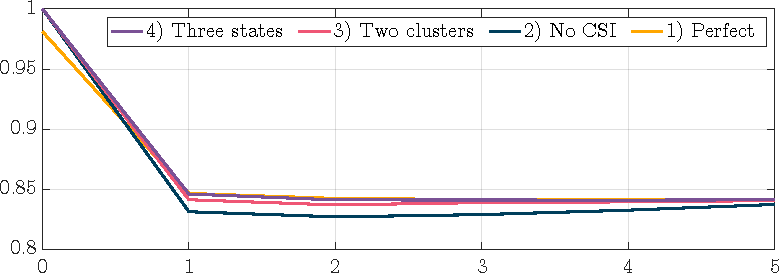
\includegraphics[width=\columnwidth]{./stability-cntrl-3.pdf}
\caption{$\rho(\mathit{\Lambda})$ from \eqref{eq:Lambda} as a function of the number of future control inputs $n_f$.}\label{fig:stability}
\end{center}
\end{figure}
\begin{figure}
\begin{center}
\vspace{-1.5mm}
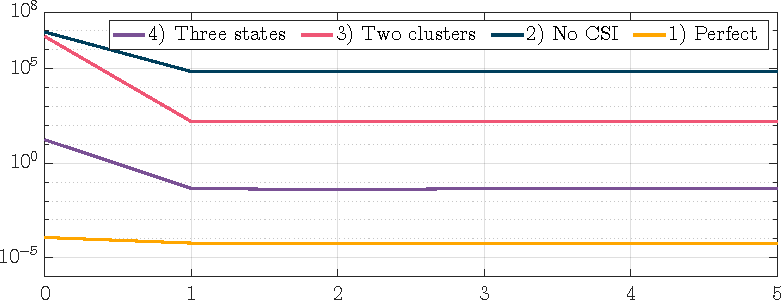
\includegraphics[width=\columnwidth]{./cost-cntrl-3.pdf}
\caption{The long-run average cost $J_{\infty}^{\star}$ from \eqref{eq:lmi-cost} as a function of the number of future control inputs $n_f$.}\label{fig:cost}
\vspace{-2mm}
\end{center}
\end{figure}

\section{Conclusions}\label{sec:conclusions}
This letter solved the wireless LQR %linear–quadratic regulation 
problem in a highly general, unconstrained setting, which considers transmitting the current and future control inputs and scaling inputs to actuators when necessary. Possible future work includes addressing constrained and output-feedback control issues and optimizing message dropout compensation parameters.
%%%%%%%%%%%%%%%%%%%%%%%%%%%%%%%%%%%%%%%%%%%%%%%%%%%%%%%%%%%%%%%%%%%%%%%%%%%%%%%%

\bibliographystyle{IEEEtran}
\bibliography{biblio}

\end{document}
